\documentclass[aspectratio=169]{beamer}
\beamertemplatenavigationsymbolsempty
\usetheme{Boadilla}
\usepackage{textpos} % package for the positioning
\usepackage{enumitem}
\usepackage{amsmath,amsfonts,amssymb}

\definecolor{uwopurple}{RGB}{79,38,131} % official purple color for uwo

\title{Foundations of Quantum Computing}
\author[]{Zyad Altahan (50238152) \and \AA{AAAAAAAAAA AAAAAAA}{6} (\AA{AAAAAAAA}{10}) \and Tobias Mette (3105540) \and Aksa Aksa (50146305)}
\institute[]{Department of Computer Science \\ University of Bonn}
\date{\today}

\usepackage[listings,many]{tcolorbox}
\makeatletter
\newtcblisting{mylisting}{
  listing only,
  breakable, enhanced jigsaw,
  listing engine=listings,
  colback=gray!20,
  listing options={
    language=python,
    keywordstyle=\color{blue},
    basicstyle=\ttfamily,
    stringstyle=\color{ForestGreen},
    commentstyle=\color{gray},
    ndkeywordstyle={\color{orange}},
    identifierstyle=\color{black},
    numbers=none,
    showstringspaces=false,
    aboveskip={0\p@ \@plus 6\p@}, belowskip={0\p@ \@plus 6\p@},
    columns=fullflexible, keepspaces=true,
    breaklines=true, breakatwhitespace=true,
    extendedchars=false,
    inputencoding=utf8,
    upquote=true,
    xleftmargin=-25pt,
  }
}
\makeatother

% set color
\setbeamercolor{title in head/foot}{bg=white}
\setbeamercolor{author in head/foot}{bg=white}
\setbeamercolor{date in head/foot}{fg=uwopurple}
\setbeamercolor{date in head/foot}{bg=white}
\setbeamercolor{title}{fg=uwopurple}
\setbeamerfont{title}{series=\bfseries}
\setbeamercolor{frametitle}{fg=uwopurple}
\setbeamerfont{frametitle}{series=\bfseries}
\setbeamercolor{block title}{bg=uwopurple!30,fg=black}
\setbeamercolor{item}{fg=uwopurple}
\setbeamercolor{caption name}{fg=uwopurple!70!}
\usefonttheme[onlymath]{serif}

\begin{document}


\begin{frame}
    \titlepage
    \begin{textblock*}{8cm}(5.0cm,-7.0cm)
        {\large \color{uwopurple}\hspace{0.66cm} \textbf{Exercise Sheet 01}} % Change the lecture # right here!
    \end{textblock*}
\end{frame}


\begin{frame}{Task 1.1: Bit string length}
    a) If $x$ is 0 or 1, the length of its binary string is 1.
    Otherwise it's the number of times $x$ can be divided by 2 (using integer division), until it reaches zero.

    Alternatively we can use the base 2 logarithm of $x$, which computes the same thing, but in a more analytical way.
    \[ \lfloor\log_2(x)\rfloor + 1\]
    This method gives us a constant running time, but the case of $x=0$ has to be handled separately.
\end{frame}

\begin{frame}[fragile]{Task 1.1: Binary vectors}
    b) A binary number can be constructed bit by bit, with successive divisions by 2, storing the remainder each time.
    But because we're using \texttt{numpy}, we can also take a vector of all powers of 2 until $n$,
    and use a single bitwise AND operation with that vector and $x$.
    \begin{mylisting}
        def binary_vector(x, n):
            index_set = np.flip(np.arange(n))
            powers_of_two = 1 << index_set
            sum_components = powers_of_two & index_set
            return np.where(sum_components != 0, 1, 0)
    \end{mylisting}
\end{frame}

\begin{frame}{Task 1.1: Output table}
    \begin{tabular}{c|c}
        $x$ & $b(x)$ \\\hline
        0 & 00000 \\
        1 & 00001 \\
        2 & 00010 \\
        3 & 00011 \\
        4 & 00100 \\
        5 & 00101 \\
        6 & 00110 \\
        7 & 00111 \\
        8 & 01000 \\
        9 & 01001 \\
       10 & 01010 \\
    \end{tabular}\hfill
    \begin{tabular}{c|c}
       $x$ & $b(x)$ \\\hline
       11 & 01011 \\
       12 & 01100 \\
       13 & 01101 \\
       14 & 01110 \\
       15 & 01111 \\
       16 & 10000 \\
       17 & 10001 \\
       18 & 10010 \\
       19 & 10011 \\
       20 & 10100 \\
       21 & 10101 \\
    \end{tabular}\hfill
    \begin{tabular}{c|c}
       $x$ & $b(x)$ \\\hline
       22 & 10110 \\
       23 & 10111 \\
       24 & 11000 \\
       25 & 11001 \\
       26 & 11010 \\
       27 & 11011 \\
       28 & 11100 \\
       29 & 11101 \\
       30 & 11110 \\
       31 & 11111 \\
       \\
    \end{tabular}
\end{frame}

\begin{frame}{Task 1.2: Grey code}
    \noindent
    \begin{minipage}[c]{0.7\linewidth}
        a) Hamming Distance is always exactly 1 between two consecutive numbers. It helps reducing distortion in communication.
        \vspace{1em}

        b) The Grey code can be easily computed by XOR-ing the number with a right-shifted copy of itself.
        \[\operatorname{grey}(x) = x \oplus (x \gg 1)\]
    \end{minipage}\hfill
    \begin{minipage}[t]{0.25\linewidth}
        \begin{tabular}{c|c|c}
            $x$ & $b(x)$ & $g(x)$ \\\hline
            0 & 000 & 000 \\
            1 & 001 & 001 \\
            2 & 010 & 011 \\
            3 & 011 & 010 \\
            4 & 100 & 110 \\
            5 & 101 & 111 \\
            6 & 110 & 101 \\
            7 & 111 & 100 \\
        \end{tabular}
    \end{minipage}
\end{frame}


\begin{frame}{Task 1.3: Cellular automata}

We simulated the evolution of a one-dimensional cellular automaton (CA) using Wolfram's rules, where a rule defines how a cell's state changes based on its current state and its neighbors. The goal was to visualize the automaton’s evolution for different rules (total possible rules: 256).

\vspace{1em}
\textbf{Approach}
\vspace{1em}
{\footnotesize
\begin{itemize}
    \item \textbf{Converted Rule to Binary}: We used a function to convert the rule number into an 8-bit binary representation to handle all possible cell configurations.
    \item \textbf{Applied Rules to Cells}: For each cell, the rule was applied based on its neighbors (left, center, right) to determine the next state.
    \item \textbf{Handled Periodic Boundaries}: We used modulo operations to simulate wrapping, allowing the grid to behave as if it were infinite.
    \item \textbf{Initialized Random Grid}: The automaton started with a randomly initialized grid of cells.
    \item \textbf{Simulated Evolution}: We iterated over time steps, updating the grid according to the rule for each cell.
\end{itemize}
}
\end{frame}

\begin{frame}{Task 1.3: Results}
\begin{columns}
    \begin{column}{0.5\textwidth}
        % Left Column Content
        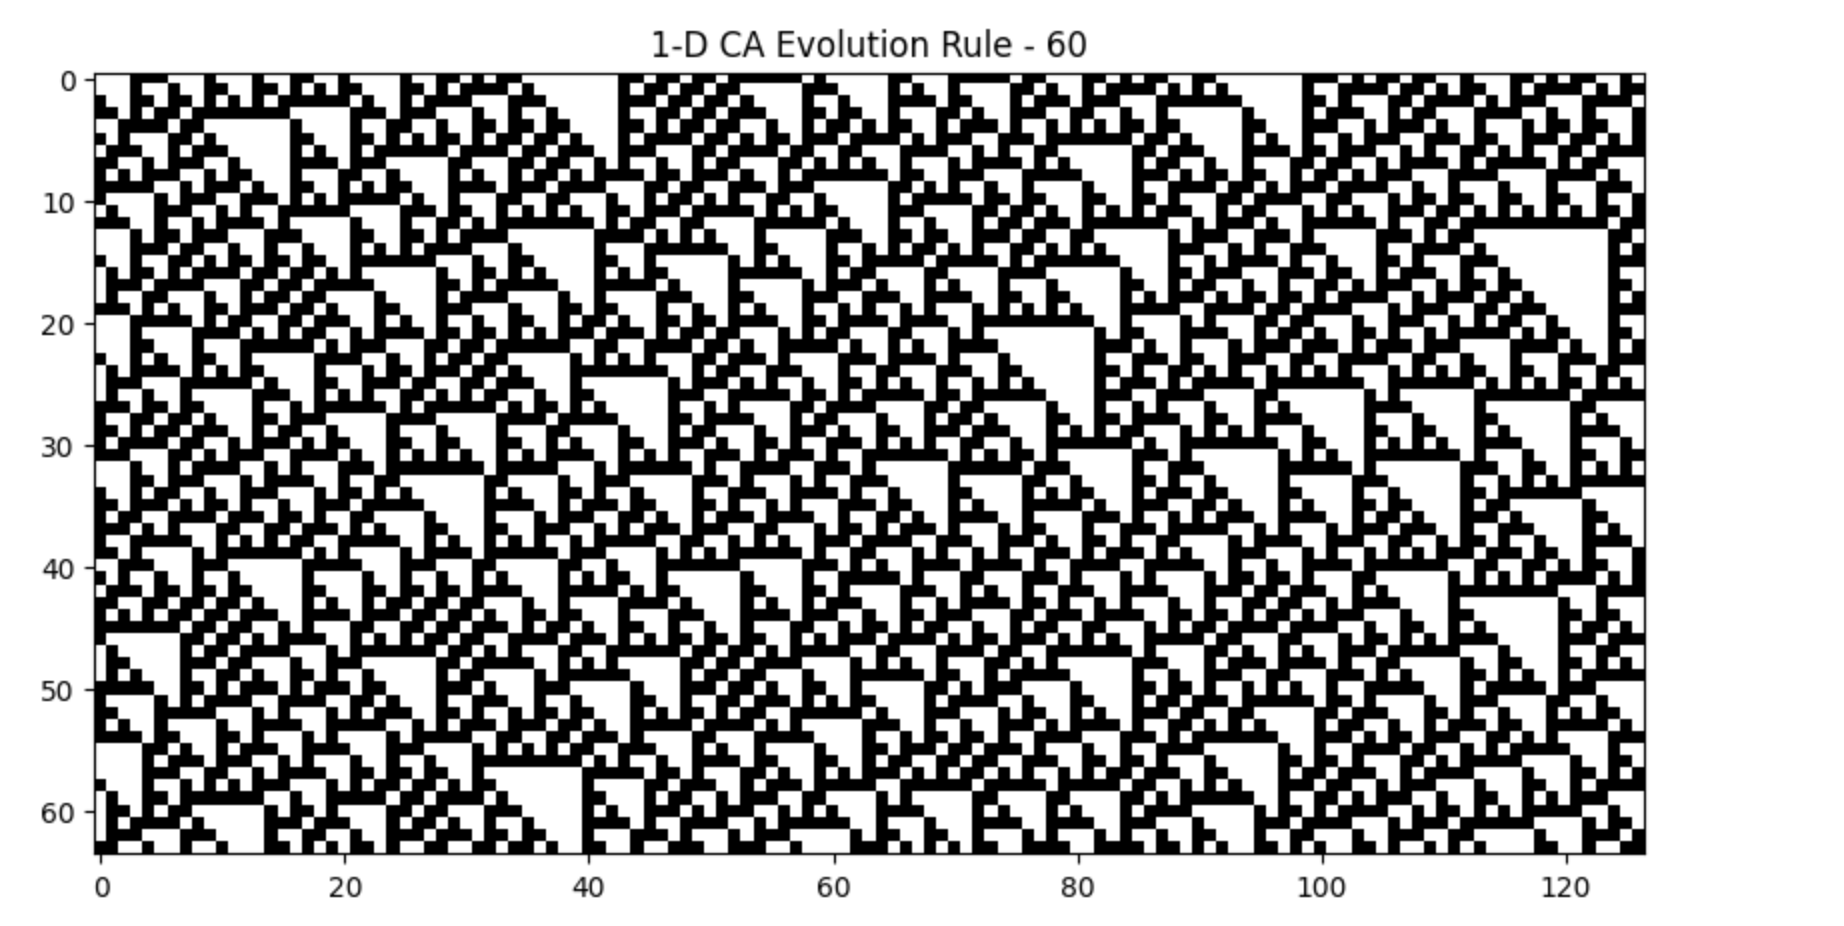
\includegraphics[width=08cm, height=06cm]{sheet01/task_1.3_rule_60.png}
    \end{column}
    \begin{column}{0.5\textwidth}
        % Right Column Content
        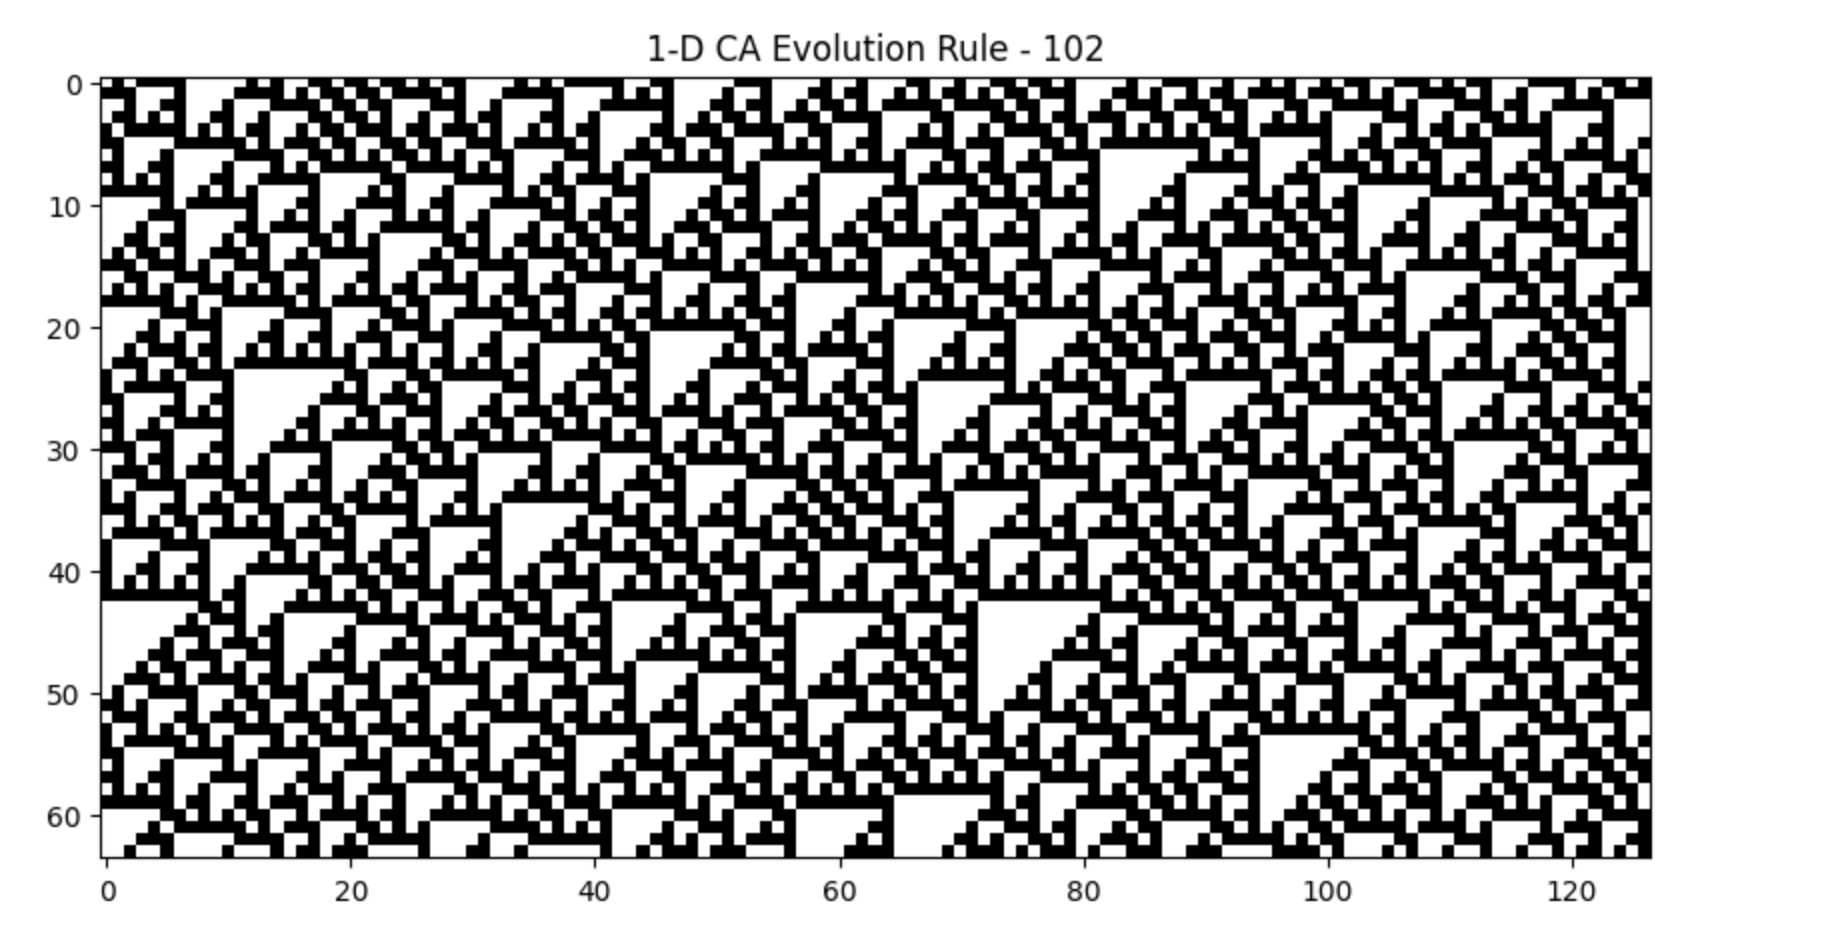
\includegraphics[width=08cm, height=06cm]{sheet01/task_1.3_rule_102.png}
    \end{column}
\end{columns}
\end{frame}


\begin{frame}{Task 1.4: Bipolar representations}
The task involved converting cellular automaton rules (specifically rules 110 and 126) into bipolar representations and then solving a least squares problem to approximate the rules with a linear model.

{\footnotesize
\vspace{1em}
\textbf{Approach}
\begin{itemize}
    \item We converted the rule numbers into an 8-bit binary format and then mapped each bit to bipolar values (0 to +1 and 1 to -1).
    \item {We used the target output \( y \) and matrix \( X^T \) to solve the least squares problem to find the weights that minimized the error between the predicted \( \hat{y} \) values and the actual \( y \) values. This was achieved using NumPy's \texttt{np.linalg.lstsq()} function.}
\end{itemize}

\textbf{Results}
The results show that for rule 110, the predicted values significantly deviate from the actual y, indicating that a linear model fails to approximate the rule effectively. For rule 126, the predicted values are nearly zero, leading to large discrepancies from the original, which shows the nonlinear nature of this rule.
Overall, both rules exhibit nonlinear behavior, as the least squares solution does not closely match the original values in either case.
}
\end{frame}

\begin{frame}{Task 1.4: Results}
\begin{columns}
    \begin{column}{0.42\textwidth}
        % Left Column Content
        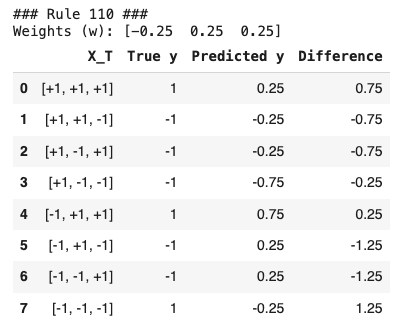
\includegraphics[width=7cm, height=7cm]{sheet01/task_1.4_rule_110.png}
    \end{column}
    \begin{column}{0.57\textwidth}
        % Right Column Content
        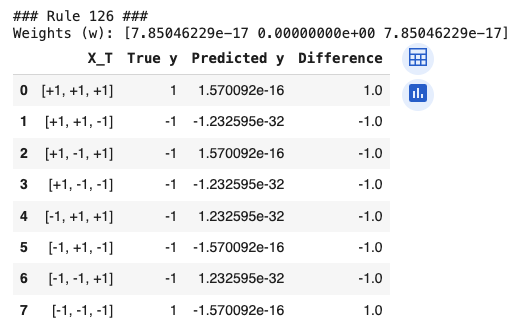
\includegraphics[width=9cm, height=7cm]{sheet01/task_1.4_rule_126.png}
    \end{column}
\end{columns}
\end{frame}

\begin{frame}[fragile]{Task 1.5: Boolean Fourier transform}
\begin{columns}
    \begin{column}{0.70\textwidth}
        To produce the desired output vector,
        we need to compute the product of all possible subsets of $x$.

        The \texttt{itertools.combinations} function provides them in the correct order, but requires a length.
        Thus we can simply supply all possible subset lengths in the range $[0, n]$.

        \begin{mylisting}
    for i in range(n+1):
        for comb in itertools.combinations(x, i):
            output.append(np.prod(comb))
        \end{mylisting}
    \end{column}
    \begin{column}{0.25\textwidth}
        \[ \varphi(x) =
        \begin{bmatrix}
        1 \\
        x_1 \\
        x_2 \\
        x_3 \\
        x_1 x_2 \\
        x_1 x_3 \\
        x_2 x_3 \\
        x_1 x_2 x_3 \\
        \end{bmatrix} \]
    \end{column}
\end{columns}
\end{frame}

\begin{frame}{Task 1.6: Approach}

\textbf{1)} Calculate $\Phi^T = $
$\begin{bmatrix}
\varphi^T_0\\
\varphi^T_1\\
\vdots\\
\varphi^T_7\\
\end{bmatrix} =
\begin{bmatrix}
\varphi^T(x_0)\\
\varphi^T(x_1)\\
\vdots\\
\varphi^T(x_7)\\
\end{bmatrix}$
with the function $\varphi(x)$ from Task 1.5.\newline

\textbf{2)} Insert $\Phi^T$ into the solution from Task 1.4 to solve the LMS-Problem.\newline\newline

$\bullet$ $x_j \in \mathbb{B}^n,$ $X^T \in \mathbb{B}^{mxn}\Rightarrow \varphi(x_j) \in \mathbb{B}^{2^n},$ $\Phi^T \in \mathbb{B}^{mx2^n}$\newline

$\bullet$ \textbf{LMS-runtime:} $\mathcal{O}(mn^2)\Rightarrow \mathcal{O}(m(2^n)^2) = \mathcal{O}(m^{3})$ because m = $2^n$

\end{frame}

\begin{frame}{Task 1.6: Results}
\begin{columns}
    \begin{column}{0.5\textwidth}
        % Left Column Content
        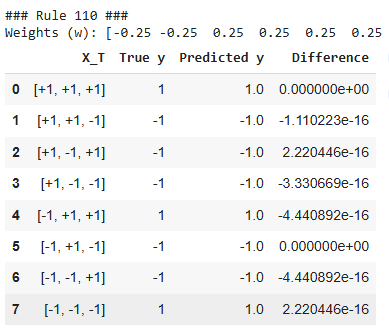
\includegraphics[width=07cm, height=07cm]{sheet01/task_1.6_rule_110.png}
    \end{column}
    \begin{column}{0.5\textwidth}
        % Right Column Content
        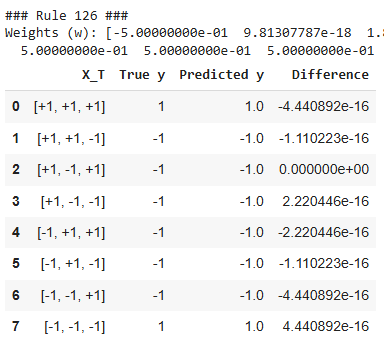
\includegraphics[width=07cm, height=07cm]{sheet01/task_1.6_rule_126.png}
    \end{column}
\end{columns}
\end{frame}


\begin{frame}{Task 1.7: Subset sum problem}

    \begin{itemize}
        \item \textbf{Sorting:}
        \begin{itemize}
            \item As all the numbers are smaller than 1000, and the target value, \( \text{trgt} = 8364 \) should be achieved.
            \item We will be using this info. to sort the array \( \text{vecX} \) in descending order, allowing the algorithm to start with larger values and improve efficiency in subset generation.
        \end{itemize}

        \item \textbf{Recursive Function Definition for Subset Generation:}
        \begin{itemize}
            \item A recursive function, \( \text{gen\_all}(\text{indices}, i) \), generates all combinations of indices for subsets of a variable size (21 in our example).
            \item Each subset's indices are stored in \( \text{indices\_set} \) to calculate their sum later on.
        \end{itemize}

        \item \textbf{Subset Summation and Target Comparison:}
        \begin{itemize}
            \item For each combination of indices, the subset sum of \( \text{vecX} \) at those indices is computed.
            \item If the subset sum equals \( \text{trgt} \), the subset values are printed.
        \end{itemize}
    \end{itemize}

\end{frame}

\begin{frame}[fragile]{Task 1.7: Code}
    Generate combinations starting from the largest numbers
    \begin{mylisting}
    vecX = np.sort(vecX)[::-1]

    indices_set = []
    comb_size = 21
    def gen_all(indices, i):
      indices_set.append(indices)
      for j in range(i, comb_size):
        gen_all(indices + [j], j+1)

    gen_all([], 0)
    ...
    if np.sum(vecX[el]) == trgt:
        print(vecX[el])
    \end{mylisting}

\end{frame}

\begin{frame}{Task 1.7: Results}
In around 14 seconds, we get 63 different set of numbers:
\begin{figure}
    \centering
    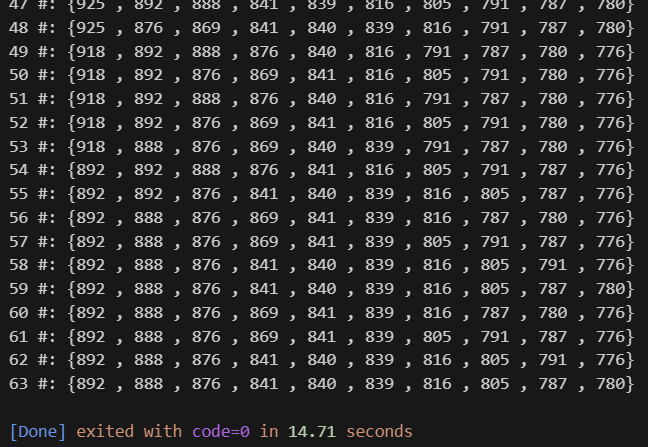
\includegraphics[width=0.66\linewidth]{sheet01/1.7-results.PNG}
    \label{fig:enter-label}
\end{figure}
\end{frame}

\end{document}
